% Created 2026-04-22 Wed 22:24
% Intended LaTeX compiler: lualatex
\DocumentMetadata{lang = en, pdfversion = 2.0, pdfstandard = ua-2, pdfstandard = a-4, testphase = {phase-III, title, table, math, firstaid}}
\documentclass[11pt]{article}
\usepackage{amsmath}
\usepackage{fontspec}
\usepackage{graphicx}
\usepackage{longtable}
\usepackage{wrapfig}
\usepackage{rotating}
\usepackage[normalem]{ulem}
\usepackage{capt-of}
\usepackage{hyperref}
\usepackage[margin=1in]{geometry}
\usepackage{fontspec}
\usepackage{verbatim, multicol, tabularx,}
\usepackage{amsmath, amsthm, amssymb, stmaryrd, latexsym, bm, listings, qtree}
\usepackage{framed}
\usepackage{xcolor,colortbl}
\usepackage{media9}
\usepackage[export]{adjustbox}
\usepackage{algorithm}
\usepackage[noend]{algpseudocode}
\usepackage{tikz,pgfplots}
\usetikzlibrary{shapes.geometric}
\let\oldquote=\quote
\let\endoldquote=\endquote
\colorlet{shadecolor}{cyan!15}
\renewenvironment{quote}{\begin{shaded*}\begin{oldquote}}{\end{oldquote}\end{shaded*}}
% From https://tex.stackexchange.com/questions/7032/good-way-to-make-textcircled-numbers
\newcommand*\circled[1]{\tikz[baseline=(char.base)]{\node[shape=circle,draw,inner sep=2pt] (char) {#1};}}
\DeclareMathOperator*{\argmin}{arg\!min}
\DeclareMathOperator*{\argmax}{arg\!max}
\lstset{frame=tb, aboveskip=1mm, belowskip=0mm, showstringspaces=false, columns=flexible, basicstyle={\scriptsize\ttfamily}, numbers=left, frame=single, breaklines=true, breakatwhitespace=true}
\hypersetup{colorlinks=true,urlcolor=blue}
\usepackage{polyglossia}
\setdefaultlanguage[variant=US]{english}
\author{Christopher Simpkins}
\date{Kennesaw State University}
\title{Artificial Intelligence\\\medskip
\large Uncertainty}
\hypersetup{
 pdfauthor={Christopher Simpkins},
 pdftitle={Artificial Intelligence},
 pdfkeywords={},
 pdfsubject={Artificial Intelligence Uncertainty},
 pdfcreator={Emacs 30.2 (Org mode 9.7.11)}, 
 pdflang={English}}
\begin{document}

\maketitle
\section{Acting Under Uncertainty}
\label{sec:org9f94d89}

Logical agents maintain a belief state and generate contingency plans that account for every possibility.  This breaks down for nontrivial problems due to:

\begin{itemize}
\item Exhaustivity of belief state, which must contain all possible states, even unlikely states.
\item Exhaustivity of contingency plan, which must account for every possible, however unlikely, action outcome.
\item Unsatisfiabilty.  There may be no guaranteed plan to achieve the goal.  If we must act anyway, how do we choose the best plan?
\item Qualification problem.  The closed-world assumption allows us to simplify logical environment specifications for simple domains, but real-world domains contain far more detail which must be accounted for.
\end{itemize}
\section{From Logic to Probability Theory}
\label{sec:org7ca5a1e}

Consider:

\begin{equation*}
Toothacke \implies Cavity
\end{equation*}

Not all patients with toothaches have cavities.  How about:

\begin{equation*}
Toothache \implies Cavity \lor GumProblem \lor Abscess \dots
\end{equation*}

We'd need large list after the dots.  Try causal direction:

\begin{equation*}
Cavity \implies Toothache
\end{equation*}

But not all cavities hurt.  Logic fails to deal with complex domains like medical diagonosis due to:

\begin{itemize}
\item \textbf{Exhaustivity} (laziness).  Too many antecedents or consequents to list.
\item \textbf{Theoretical ignorance}. Rare to have complete logical theory of nontrivial domain.
\item \textbf{Practical ignorance}.  Even with a complete domain theory, hard to measure all the necessary inputs (medical tests, etc.)
\end{itemize}

We need to deal with uncertain knowledge, with \textbf{degrees of belief}.  For that, we use probability theory.
\section{Probability Theory as Knowledge Representation}
\label{sec:orgf307239}

\begin{itemize}
\item Ontological commitments of logic and probability theory same:

\begin{itemize}
\item World composed of facts that do or do not hold in any particular case.
\end{itemize}

\item Epistemological commitments differ:

\begin{itemize}
\item Logic assigns true, false, or no opinion to each sentence.
\item Probability theory assignesnumerical degree of belief between 0 (for sentences that are certainly false) and 1 (certainly true) to each sentence.
\end{itemize}
\end{itemize}

Probability theory solves the qualification problem by summarizing the uncertainty stemming from our laziness and ignorance.
\section{What do probabilities mean?}
\label{sec:orgc4c2306}


\includegraphics[alt={neo architect prob dist screens},width=0.75\linewidth]{neo-architect-prob-dist-screens.png}
\section{Probabilities are about our uncertain knowledge.}
\label{sec:org3842f47}

"80\% chance (probability 0.8) patient with a toothache has a cavity."

\begin{itemize}
\item Out of all the situations that are indistinguishable from the current situation \textbf{as far as our knowledge goes}, the patient will have a cavity in 80\% of them.
\item Belief could come from statistical data, or domain theory, or combination of sources.
\end{itemize}

\begin{quote}
There is no uncertainty in the actual world.  The patient either has a cavity or does not. Probabilities refer to our knowledge of the world state, not the actual world state.
\end{quote}

If our knowledge changes, e.g., we find out patient has history of gum disease, we make a different statement.

"Given patient has a history of gum disease and a toothache, 40\% chance patient has gum disease."
\section{Rational Decisions}
\label{sec:org5b4e270}

How do we choose between different plans that acheive the goal?

\begin{itemize}
\item Each plan has a likelihood of success, e.g.:

\begin{itemize}
\item Plan A has a 95\% chance of achieving a goal state.
\end{itemize}

\item Each plan may lead to goal states with different outcomes, each of which is a goal state.

\begin{itemize}
\item An \textbf{outcome} of an action is a completely specified state, which includes elements that are not part of the goal.
\end{itemize}
\end{itemize}

Elements of outcomes can be more or less desirable -- more or less \textbf{useful} -- to a given agent.

\begin{itemize}
\item Utility is the quality of being useful.
\item That "usefulness" may simply be pleasure, or even altruism.
\end{itemize}

Utility theory associates a utility value with each possible outcome, which induces a preference ordering over outcomes.

\begin{quote}
An agent is rational if and only if it chooses the action that yields the highest expected utility, averaged over all the possible outcomes of the action.
\end{quote}
\section{Decision-Theoretic Agents}
\label{sec:orga207a7e}

\begin{quote}
Decision theory = probability theory + utility theory
\end{quote}


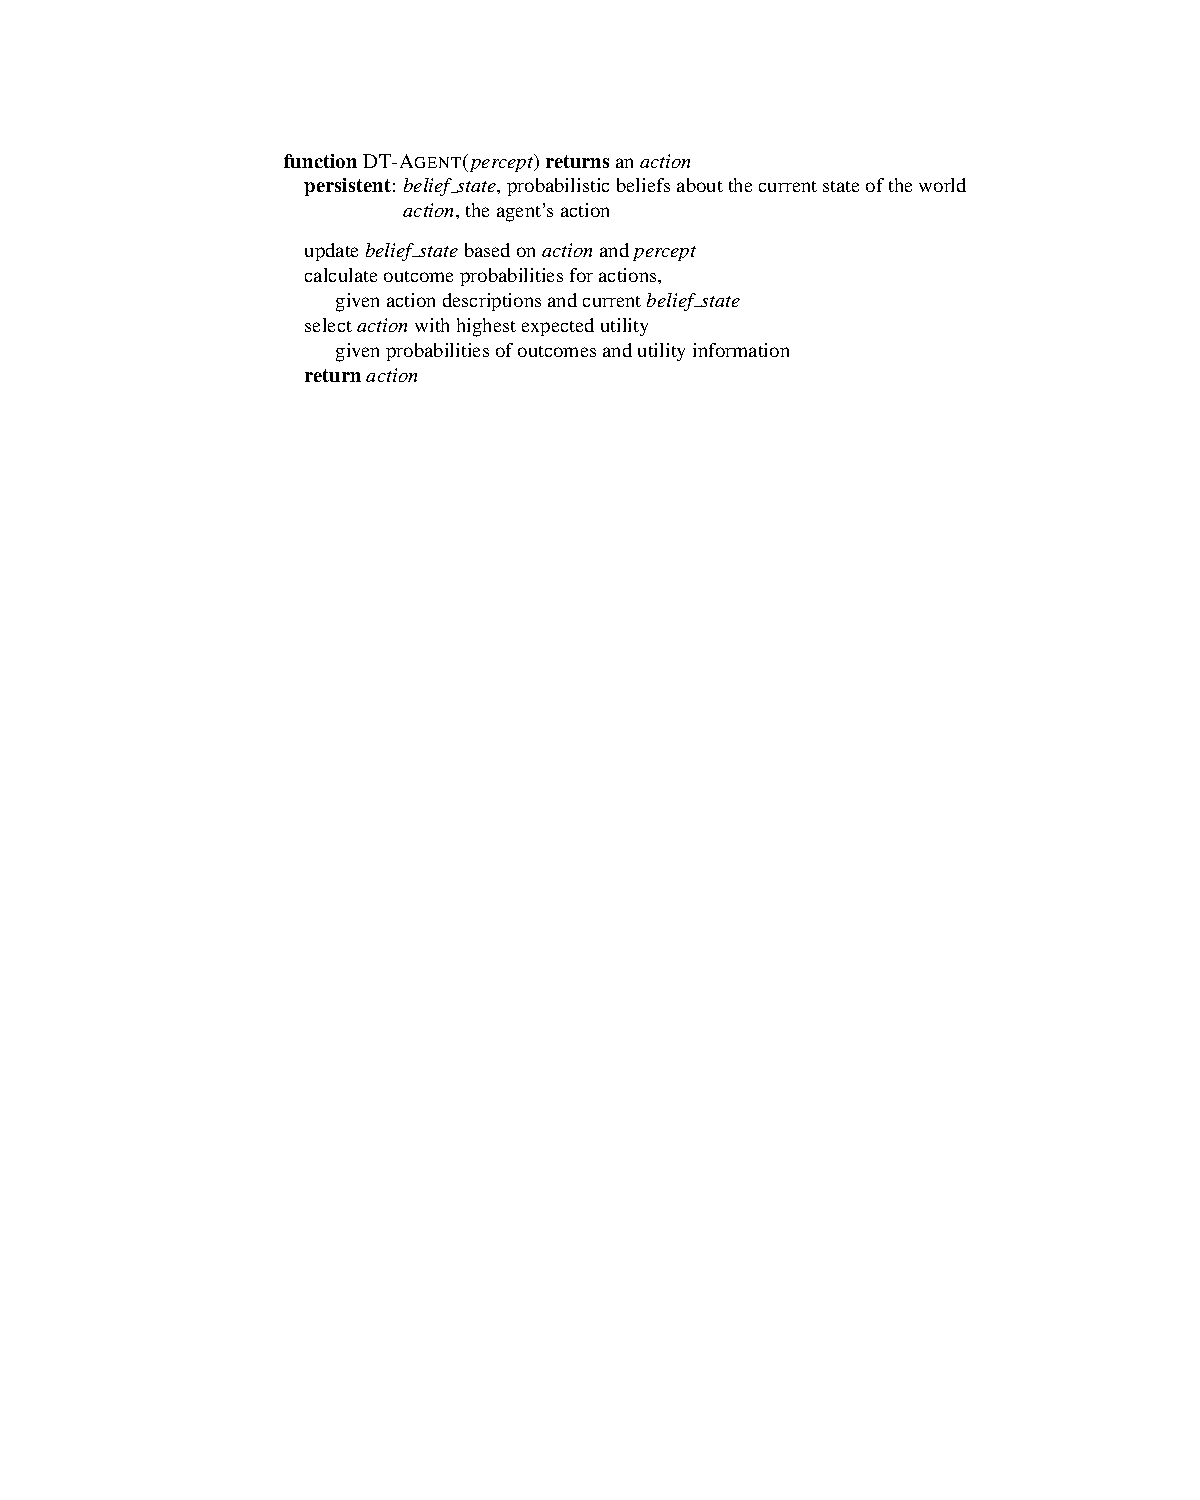
\includegraphics[alt={aima fig 12_01 dt agent algorithm},height=1.2in]{aima-fig-12_01-dt-agent-algorithm.pdf}



Each action, \(a\), leads to a probability distribution over outcomes, or "result states":

$$
P(\text{RESULT}(a) = s') = \sum_{s \in S} P(s) P(s' \mid s, a)
$$

And each outcome state has a utility.  A rational decision-theoretic agent chooses the action that maximize expected utility, that is:

$$
\argmax_{a} \sum_{s' \in S} P(\text{RESULT}(a) = s') U(s')
$$
\section{Probability Models}
\label{sec:orgda25639}

In logic we have satisfiabilty: \(M(\alpha)\) is the set of all possible worlds in which sentence \(\alpha\) is true.

In probability theory the set of possible worlds is a \textbf{sample space}, \(\Omega\), which must be mutually exclusive and exhaustive (one and only one possible world must be the case).

$$
0 \le P(\omega) \le 1 \text{ for every } \omega \text{ and } \sum_{\omega \in \Omega} P(\omega) = 1
$$

Each \(\omega\) is a possible world.  Probability textbooks typically call these outcomes.  For example, each of these pairs is a \(\omega \in \Omega\) for the roll of two dice:

\footnotesize
\begin{tabular}{cccccc}
(1, 1) & (2, 1) & (3, 1) & (4, 1) & (5, 1) & (6, 1)\\
(1, 2) & (2, 2) & (3, 2) & (4, 2) & (5, 2) & (6, 2)\\
(1, 3) & (2, 3) & (3, 3) & (4, 3) & (5, 3) & (6, 3)\\
(1, 4) & (2, 4) & (3, 4) & (4, 4) & (5, 4) & (6, 4)\\
(1, 5) & (2, 5) & (3, 5) & (4, 5) & (5, 5) & (6, 5)\\
(1, 6) & (2, 6) & (3, 6) & (4, 6) & (5, 6) & (6, 6)\\
\end{tabular}
\normalsize

In probability textbooks, an \textbf{experiment} leads to a sample space.  Here, the set of possible worlds comes from the task environment.
\section{Propositions and Events}
\label{sec:org3ba939b}

An \textbf{event}, which we denote with \(\phi\) here, is a set of possible worlds, some subset of \(\Omega\), or set of \(\omega\), e.g., the event "doubles" contains the 6 boxed elements \(\omega\):

\footnotesize
\begin{tabular}{cccccc}
\boxed{(1, 1)} & (2, 1) & (3, 1) & (4, 1) & (5, 1) & (6, 1)\\
(1, 2) & \boxed{(2, 2)} & (3, 2) & (4, 2) & (5, 2) & (6, 2)\\
(1, 3) & (2, 3) & \boxed{(3, 3)} & (4, 3) & (5, 3) & (6, 3)\\
(1, 4) & (2, 4) & (3, 4) & \boxed{(4, 4)} & (5, 4) & (6, 4)\\
(1, 5) & (2, 5) & (3, 5) & (4, 5) & \boxed{(5, 5)} & (6, 5)\\
(1, 6) & (2, 6) & (3, 6) & (4, 6) & (5, 6) & \boxed{(6, 6)}\\
\end{tabular}
\normalsize


A \textbf{proposition} is an event expressed in a formal language; specifically, for each proposition, the corresponding set contains just those possible worlds in which the proposition holds.

The probability associated with a proposition is defined to be the sum of the probabilities of the worlds in which it holds:

\begin{equation*}
\text{For any proposition } \phi, P(\phi) = \sum_{\omega \in \phi} P(\omega)
\end{equation*}

Example: \(P(Doubles) = P((1, 1)) + \cdots + P((6, 6)) = \frac{1}{36} + \cdots + \frac{1}{36} = \frac{1}{6}\)
\section{Prior and Conditional Probabilities}
\label{sec:orgf16e67a}

An \textbf{unconditional} or \textbf{prior} probability is a degree of belief in a proposition with no other information.

A \textbf{conditional} or \textbf{posterior} probability is a degree of belief in a proposition given some relevant information.

Definition of conditional probability:

\begin{equation*}
P(a  \mid  b) = \frac{P(a \land b)}{P(b)}
\end{equation*}

From that definition we get the \textbf{product rule}:

\begin{equation*}
P(a \land b) = P(a  \mid  b) P(b)
\end{equation*}

Note that \(P(a \land b)\) can also be written \(P(a,b)\) or \(P(ab)\).
\section{Conditional probability is not implication.}
\label{sec:orgd1932d5}

The assertion

\begin{equation*}
P(cavity \mid toothache) = 0.6
\end{equation*}

does not mean "Whenever toothache is true, conclude that cavity is true with probability 0.6"

It means "Whenever toothache is true \textbf{and we have no further information}, conclude that cavity is true with probability 0.6."

If we had the further information that the dentist found no cavities, certainly not the case that cavity is true with probability 0.6; instead we have

\begin{equation*}
P(cavity \mid toothache \land \neg cavity) = 0
\end{equation*}
\section{Probability Assertions}
\label{sec:org56416d2}


A \textbf{random variable}, which begins with capital letter, is a function mapping from possible worlds \(\Omega\) to a set of possible values the variable can take.

\begin{itemize}
\item \(Die_1: \{1, \dots, 6\} \to \{1, \dots, 6\}\)
\item \(Doubles: \{1, \dots, 6\} \times \{1, \dots, 6\} \to \{true, false\}\)
\item \(Weather: \{sun,rain,cloud,snow\} \to \{sun,rain,cloud,snow\}\)
\end{itemize}

Individual values are written in lowercase and often abbreviated.

\begin{itemize}
\item \(P(sun)\) stands for \(P(Weather=sun)\).
\end{itemize}

A \textbf{probability distribution} is an assignment of probabilities to all values of a rendom variable, e.g.:

\begin{align*}
P(Weather=sun)   &= 0.6 \\
P(Weather=rain)  &= 0.1 \\
P(Weather=cloud) &= 0.29 \\
P(Weather=snow)  &= 0.01
\end{align*}

Which can also be written \(P(Weather) = \langle 0.6, 0.1, 0.29. 0.01 \rangle\).
\section{Joint Probability Distributions}
\label{sec:org67bdd75}

\(P(Weather, Cavity)\) denotes the probabilities of all combinations of \(Weather\) and \(Cavity\).  This notation is a compact representation of a \textbf{joint probability distribution}.  The notation

\begin{equation*}
P(Weather, Cavity) = P(Weather  \mid  Cavity) P(Cavity)
\end{equation*}

stands for the \(4 \times 2 = 8\) equations:

\begin{align*}
P(W = sun \land C = true)    &= P(W = sun  \mid  C = true) P(C = true) \\
P(W = rain \land C = true)   &= P(W = rain  \mid  C = true) P(C = true) \\
P(W = cloud \land C = true)  &= P(W = cloud  \mid  C = true) P(C = true) \\
P(W = snow \land C = true)   &= P(W = snow  \mid  C = true) P(C = true) \\
P(W = sun \land C = false)   &= P(W = sun  \mid  C = false) P(C = false) \\
P(W = rain \land C = false)  &= P(W = rain  \mid  C = false) P(C = false) \\
P(W = cloud \land C = false) &= P(W = cloud  \mid  C = false) P(C = false) \\
P(W = snow \land C = false)  &= P(W = snow  \mid  C = false) P(C = false)
\end{align*}
\section{Probability Axioms}
\label{sec:org5040c7f}

All of probability theory can be built from \textbf{Kolmogorov's axioms}.

Law of normalization:

\begin{equation*}
0 \le P(\omega) \le 1 \text{ for every } \omega \text{ and } \sum_{\omega \in \Omega} P(\omega) = 1
\end{equation*}


Probability of a disjunction, \textbf{inclusion-exlusion principle}:

\begin{equation*}
P(a \lor b) = P(a) + P(b) - P(a \land b)
\end{equation*}
\section{Why is probability theory a valid basis for rational behavior?}
\label{sec:orgfbfa324}

De Finetti's Theorem:

\begin{quote}
If Agent 1 expresses a set of degrees of belief that violate the axioms of probability theory then there is a combination of bets by Agent 2 that guarantees that Agent 1 will lose money every time.
\end{quote}

Example:


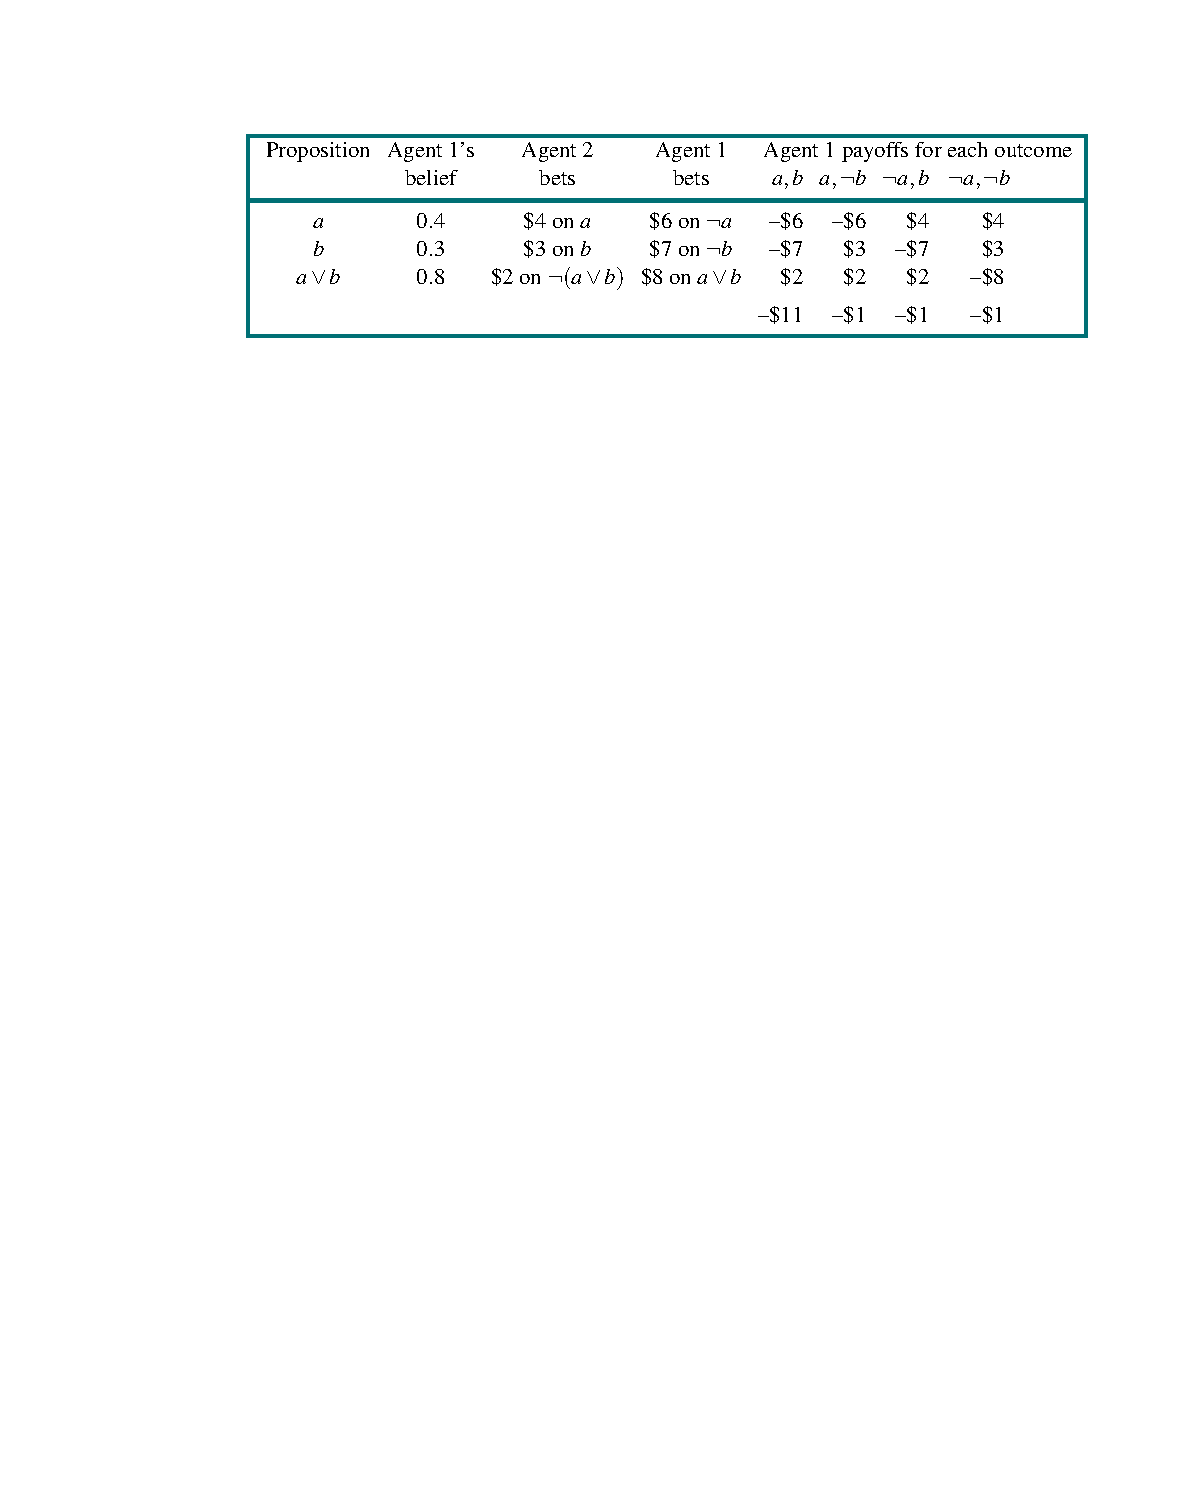
\includegraphics[alt={aima fig 12_02 agent bets},width=0.75\linewidth]{aima-fig-12_02-agent-bets.pdf}
\section{Inference Using Full Joint Distributions}
\label{sec:orga9a2e4e}

Knowledge base is full joint distribution of boolean random variables \(Toothache, Cavity, Catch\).


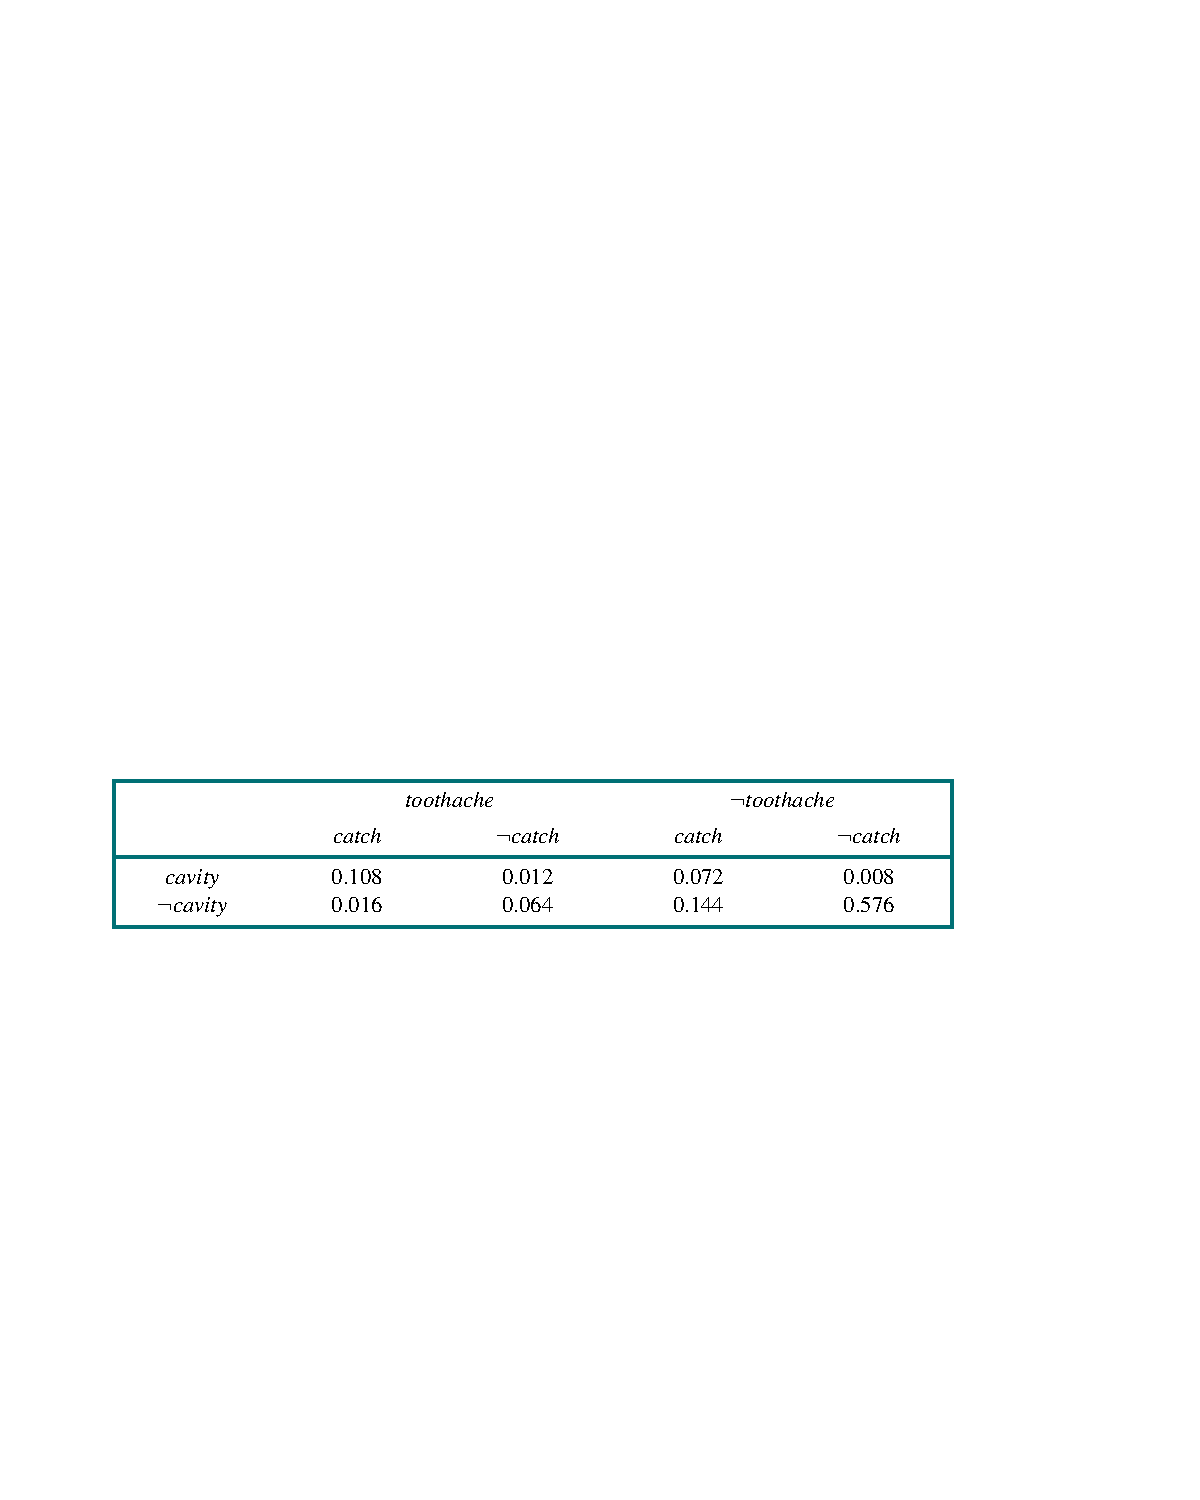
\includegraphics[alt={aima fig 12_03 full joint toothache},width=0.75\linewidth]{aima-fig-12_03-full-joint-toothache.pdf}



\begin{itemize}
\item All probabilities above sum to 1.
\item \(P(cavity \lor toothache) = 0.108 + 0.012 + 0.072 + 0.008 + 0.016 + 0.064= 0.28\).
\end{itemize}


Unconditional or \textbf{marginal probability} of cavity:

\begin{equation*}
P(cavity) = 0.108 + 0.012 + 0.072 + 0.008= 0.2
\end{equation*}
\section{Marginalization and Conditioning}
\label{sec:org6b2225c}


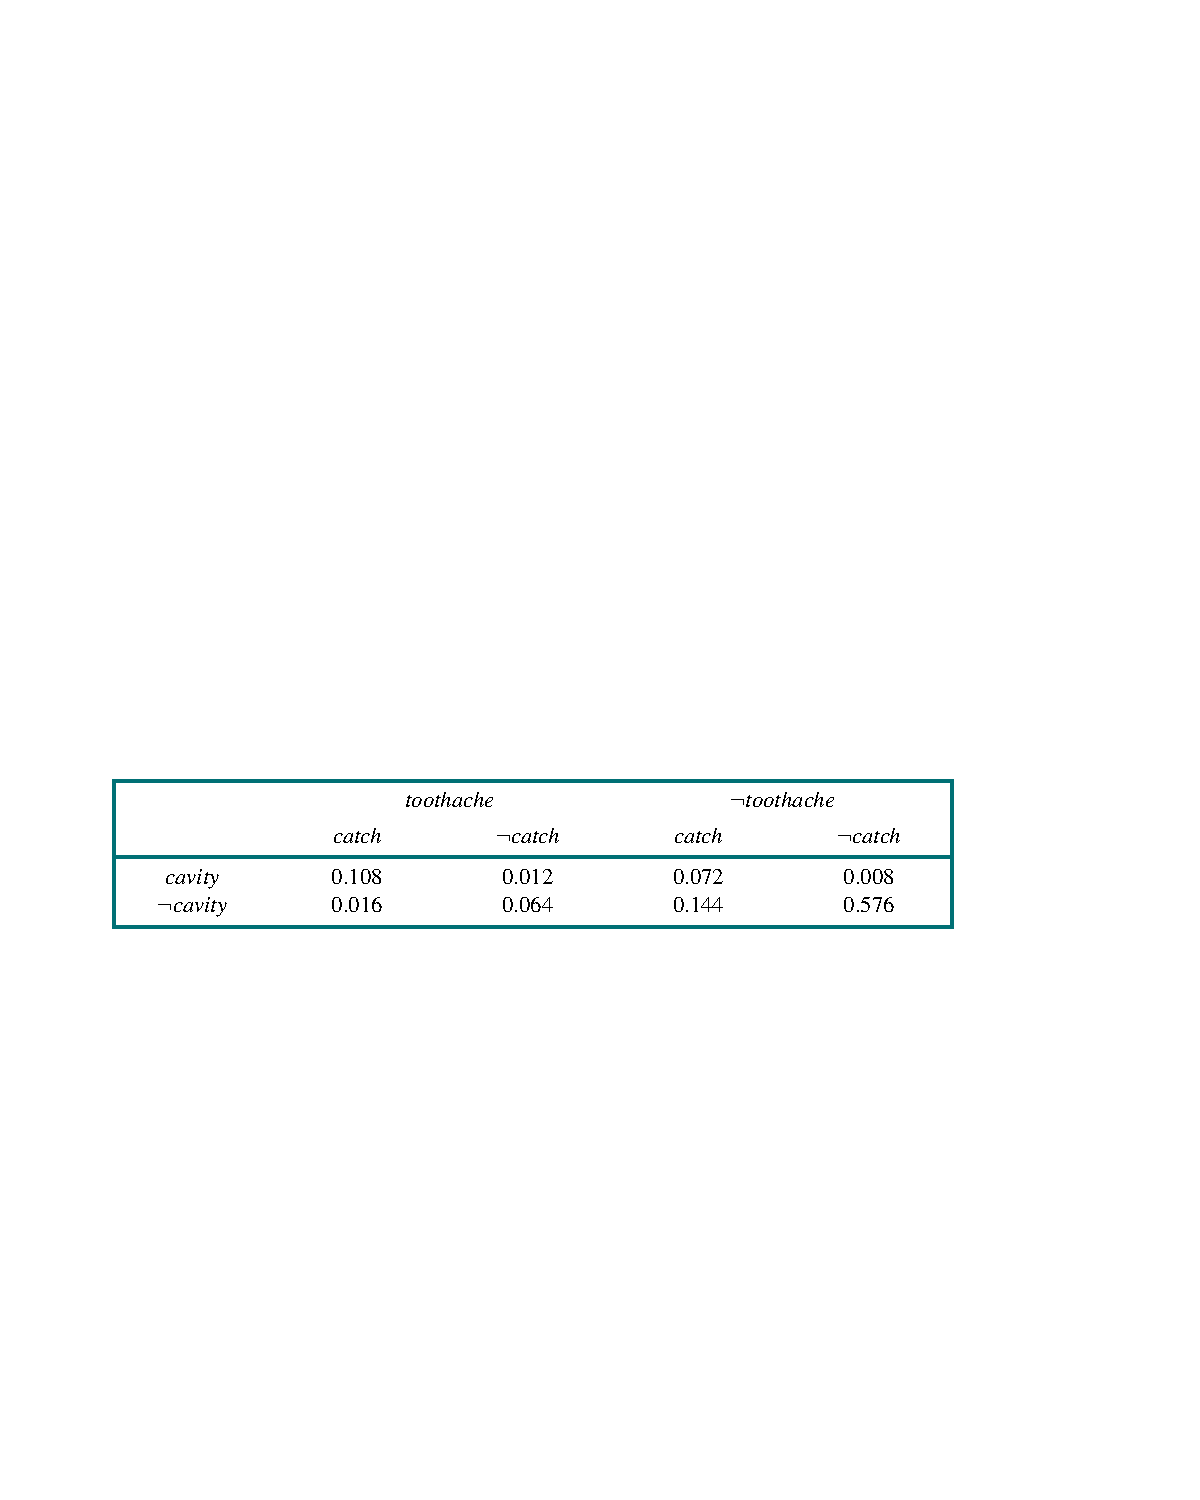
\includegraphics[alt={aima fig 12_03 full joint toothache},height=0.8in]{aima-fig-12_03-full-joint-toothache.pdf}



\textbf{Marginalization} means "summing out" the non-query variables, which we usually denote with \(Z\):

\vspace{-.1in}
\[
P(Y) = \sum_z P(Y, Z=z)
\]
\vspace{-.1in}

For example, let \(Y = Cavity\):

\vspace{-.2in}
\begin{align*}
P(Cavity) &= P(Cavity, toothache, catch) + P(Cavity, toothache, \neg catch) \\
           &+ P(Cavity, \neg toothache, catch) + P(Cavity, \neg toothache, \neg catch) \\
           &= <0.108, 0.016> + <0.012, 0.064> + <0.072, 0.144> + <0.008, 0.576>\\
           &= <0.2, 0.8>
\end{align*}
\vspace{-.1in}

Using the product rule in \(P(Y) = \sum_z P(Y, Z=z)\) we obtain the \textbf{conditioning} rule:

\vspace{-.1in}
\[
P(Y) = \sum_z P(Y \mid z) P(z)
\]
\vspace{-.1in}

These two rules are used widely in probabilistic reasoning.
\section{Condional Probability Distributions}
\label{sec:org07ffea1}

We're usually interested in conditional probabilities.  To get the conditional probabilites, we use the definition:

\begin{align*}
P(cavity  \mid  toothache) &= \frac{P(cavity \land toothache)}{P(toothache)}\\
                       &= \frac{0.108 + 0.012}{0.108 + 0.012 + 0.016 + 0.064} = 0.6
\end{align*}

\begin{align*}
P(\neg cavity  \mid  toothache) &= \frac{P(\neg cavity \land toothache)}{P(toothache)}\\
                            &= \frac{0.016 + 0.064}{0.108 + 0.012 + 0.016 + 0.064} = 0.4
\end{align*}
\section{Normalization}
\label{sec:org916106a}

Notice that \(P(toothache)\) appears in denominator in both equations in the preceding conditional probability calculations.  We can vew it as a \textbf{normalization constant}, denoted \(\alpha\), that ensures that the conditional probability distribution \(P(Cavity  \mid  toothache)\) sums to 1.  Then we can write:

\vspace{-.25in}
\begin{align*}
P(Cavity  \mid  toothache) &= \alpha P(Cavity, toothache) \\
                       &= \alpha [ P(Cavity, toothache, catch) + P(Cavity, toothache, \neg catch)] \\
                       &= \alpha [<0.108, 0.16> + <0.012, 0.064>\\
                       &= \alpha <0.12, 0.08> \\
                       &= <0.6, 0.4>
\end{align*}

The cool thing is that we don't even have to know \(P(toothache)\) to calculate the conditional probability distribution \(P(Cavity \mid toothache)\).  To make this point clearer, imagine the penultimate line above is:

\begin{equation*}
P(Cavity  \mid  toothache) = \alpha <0.3, 0.2>
\end{equation*}

What's \(\alpha\)?
\section{Inference Using the Full Joint Distribution}
\label{sec:org78d4c87}

All of the preceding can be summarized in a general inference procedure using full joint probability distributions.  Let \(E\) be a list of evidence variables, \(\bm{e}\) be a list of observed values for the evidence variables, and \(Y\) be the remaining unobserved variables.  Then:

\begin{equation*}
P(X  \mid  \bm{e}) = \alpha P(X, \bm{e}) = \alpha \sum_y P(X, \bm{e}, \bm{y}) \tag{12.9}
\end{equation*}

Great, so we're done!  All we need is a full joint probability distribution and we can answer any query.  Unfortunately, not practical.

\begin{itemize}
\item For a domain of \(n\) boolean variables, we have a table of size \(O(2^n)\)
\end{itemize}

So we need different approaches, which we cover next.
\section{Independence}
\label{sec:org7e1b6d9}

Weather is not affecteed by teeth.  So we can assert:

\begin{equation*}
P(cloud  \mid toothache,catch,cavity) = P(cloud)
\end{equation*}

In general, if \(a\) and \(b\) are independent:

\begin{equation*}
P(a \mid b) = P(a) \text{ or } P(b \mid a) = P(b) \text{ or } P(a \land b) = P(a)P(b)
\end{equation*}

Can be a big help.  For example, if you have \(n\) independent coin flips, then instead of \(2^n\) full joint table, you have a product of \(n\) distributions \(P(C_i)\).


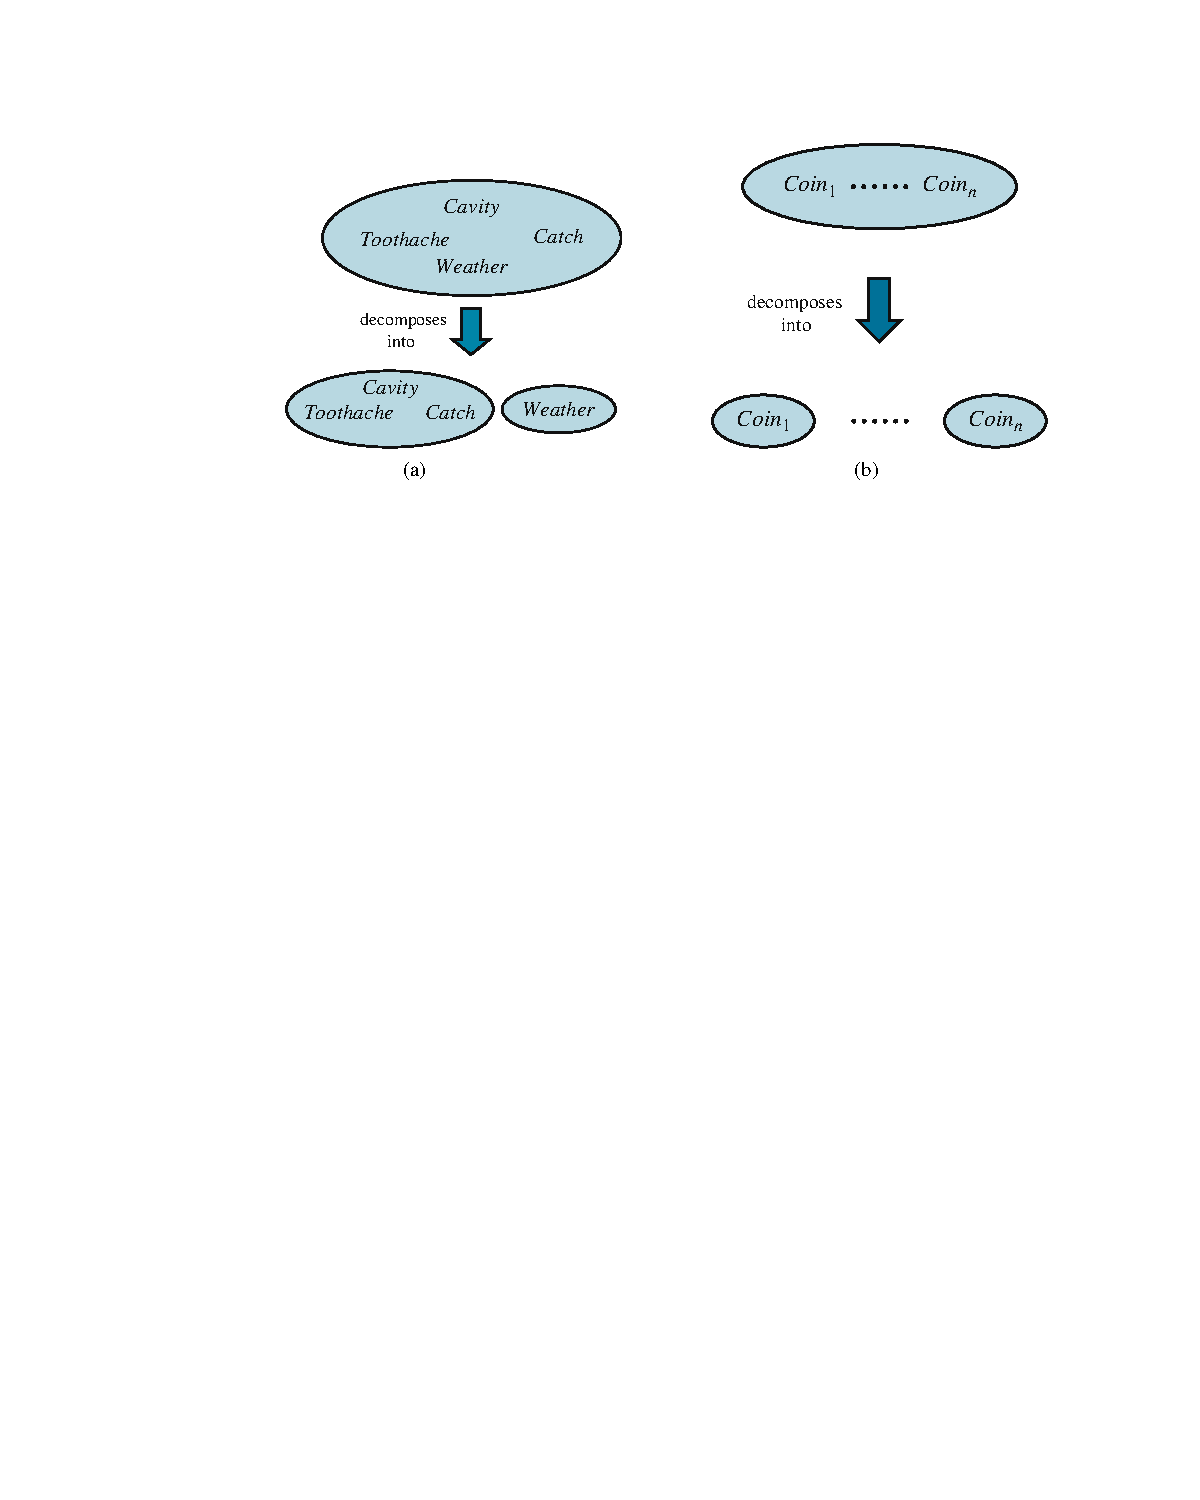
\includegraphics[alt={aima fig 12_04 factoring independence},height=1.2in]{aima-fig-12_04-factoring-independence.pdf}



Unfortunately, independence rarely holds in the real world.
\section{Bayes' Rule}
\label{sec:org8ca0f93}

Using the symmetry \(P(X, Y) = P(Y, X)\) and the product rule we can derive \textbf{Bayes' rule}:

\begin{align*}
P(X, Y)     &= P(Y, X)\\
P(Y \mid X)P(X) &= P(X \mid Y)P(Y)\\
P(Y \mid X)      &= \frac{P(X \mid Y)P(Y)}{P(X)}
\end{align*}

The usefulness of Bayes' rule becomes apparent if we consider \(X\) as an effect and \(Y\) as a cause and we want to determine the cause of some effect (evidence) we observe:

\begin{equation*}
P(\text{cause} \mid \text{effect}) = \frac{P(\text{effect} \mid \text{cause}) P(\text{cause})}{P(\text{effect})}
\end{equation*}

\begin{itemize}
\item \(P(\text{effect} \mid \text{cause})\) quantifies the \textbf{causal} direction.
\item \(P(\text{cause} \mid \text{effect})\) quantifies the \textbf{diagnostic} direction.
\end{itemize}

Reasoning from effects to causes is also called \textbf{abductive reasoning}.  (Is Sherlock Holmes truly employing deduction?)
\section{A Medical Screening Example}
\label{sec:orgc7b6b3a}

A cancer with occurence rate of 1\% (.01) has a "90\% accurate" test, and:


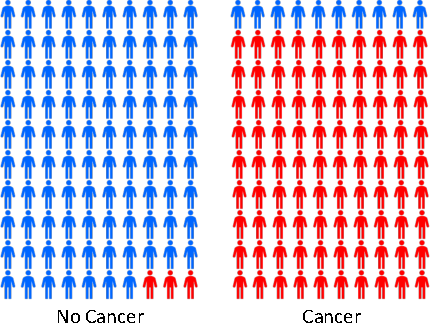
\includegraphics[alt={../../deep learning/slides/bishop dl fig2.3},height=1.8in]{../../deep-learning/slides/bishop-dl-fig2.3.pdf}



False positive rate: .03, False negative rate: 0.10


Questions:

\begin{itemize}
\item If we screen someone, what is the probability that they test positive?
\item If someone tests positive, what is the probability that they have cancer?
\end{itemize}

The test is an effect.  Cancer is the cause.
\section{Analysis of Medical Screening Example}
\label{sec:org356b53c}


With our probabilistic machinery we can analyze this cancer screening example.  First, we model the problem in the language of Bayesian probability theory:

\begin{align*}
P(C=1)     &= \frac{1}{100}  \tag{Prior probability that someone has cancer}\\
P(C=0)     &= \frac{99}{100} \tag{Prior probability that someone has no cancer}\\
P(T=1 \mid C=1) &= \frac{90}{100} \tag{Conditional probability of positive test given cancer}\\
P(T=0 \mid C=1) &= \frac{10}{100} \tag{Conditional probability of negative test given cancer}\\
P(T=1 \mid C=0) &= \frac{3}{100}  \tag{Conditional probability of positive test given no cancer}\\
P(T=0 \mid C=0) &= \frac{97}{100} \tag{Conditional probability of negative test given no cancer}
\end{align*}

Now we can answer the two questions we posed at the outset:

\begin{itemize}
\item If we screen someone, what is the probability that they test positive?
\item If someone tests positive, what is the probability that they have cancer?
\end{itemize}
\section{Analysis of Medical Screening Example}
\label{sec:org49352e3}





\begin{align*}
P(C=1)     &= \frac{1}{100} \\
P(C=0)     &= \frac{99}{100}\\
P(T=1 \mid C=1) &= \frac{90}{100}\\
P(T=0 \mid C=1) &= \frac{10}{100}\\
P(T=1 \mid C=0) &= \frac{3}{100} \\
P(T=0 \mid C=0) &= \frac{97}{100}
\end{align*}




If we screen someone, probability that they test positive (notice use of product rule: \(P(a, b) = P(a \mid b) P(b)\) and rule 2nd Kolmogorov axiom \(P(x \lor y) = P(x) + P(y) - P(x \land y)\)):

\vspace{-.1in}
\begin{align*}
P(T=1) &= P(T=1 \mid C=0)P(C=0) + P(T=1 \mid C=1)P(C=1)\\
       &= \frac{3}{100} \times \frac{99}{100} + \frac{90}{100} \times \frac{1}{100}\\
       &= \frac{387}{10,000}\\
       &= .0387
\end{align*}

If someone tests positive, probability they have cancer :

\vspace{-.1in}
\begin{align*}
P(C=1 \mid T=1) &= \frac{P(T=1 \mid C=1)P(C=1)}{P(T=1)}\\
           &= \frac{90}{100} \times \frac{1}{100} \times \frac{10,000}{387} \\
           &= \frac{90}{387}\\
           &\approx 0.23
\end{align*}
\section{Bayes' Rule and Combining Evidence}
\label{sec:org05127ae}

If dentist's probe catches and patient has a toothache, then using the full joint:



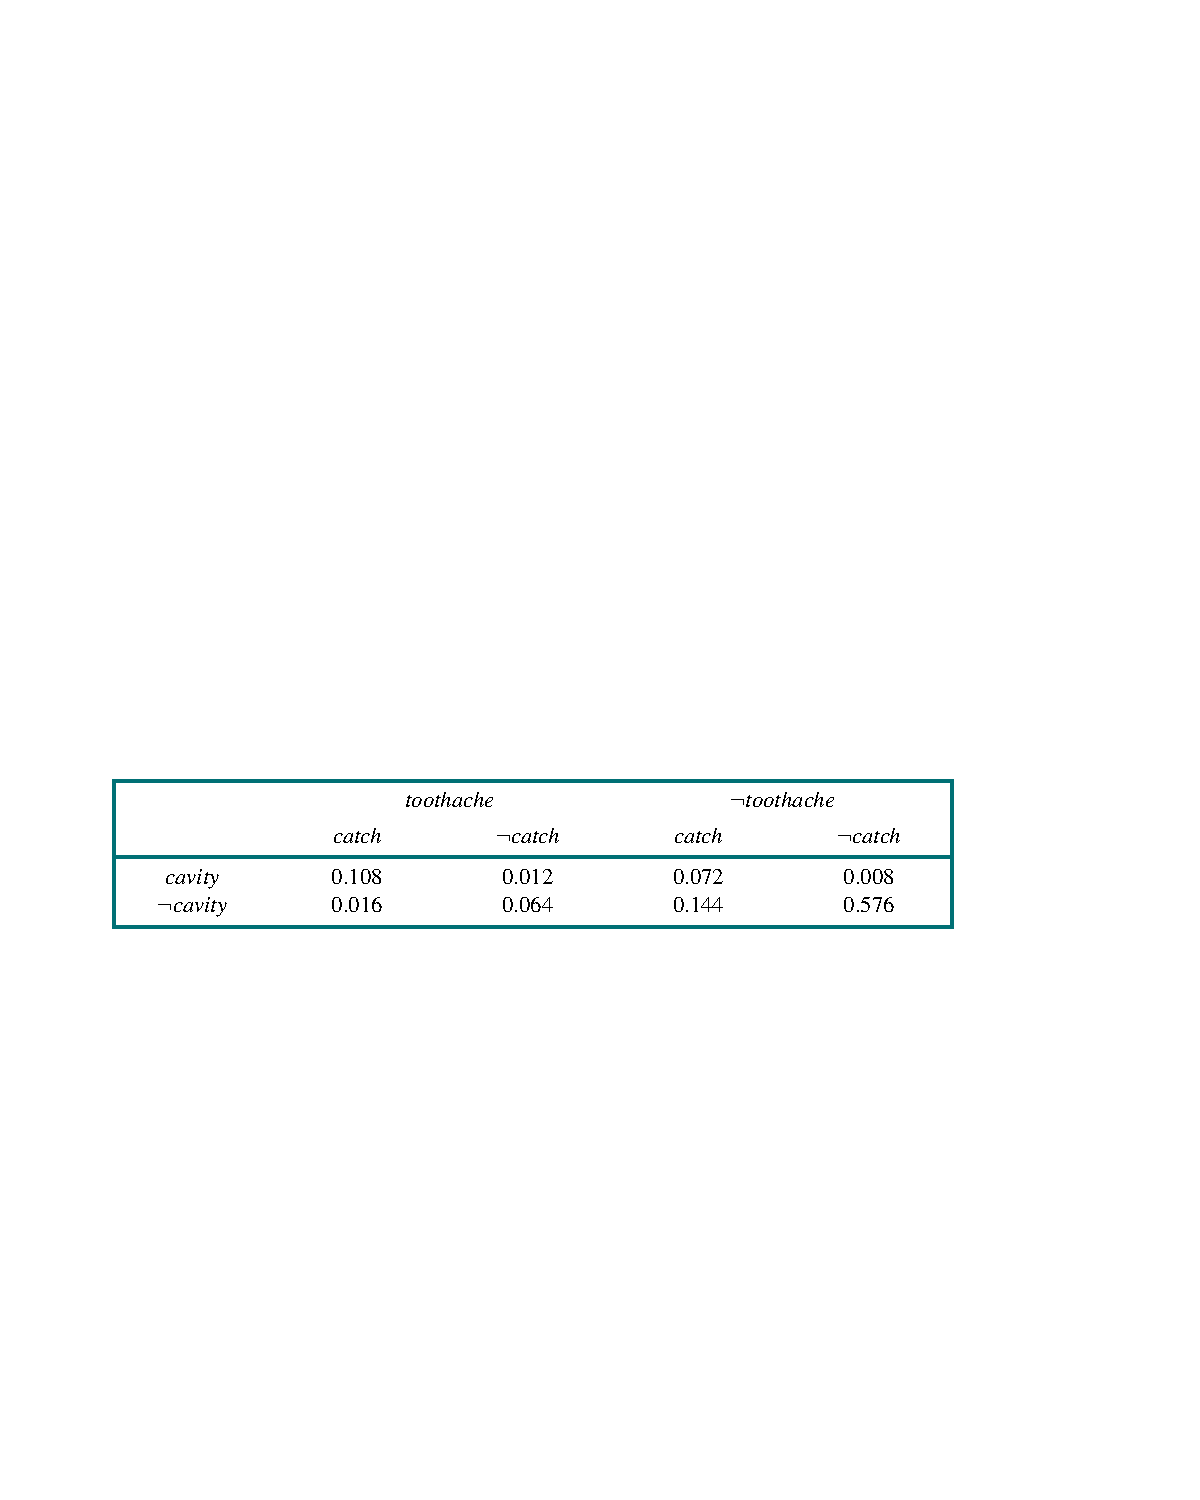
\includegraphics[alt={aima fig 12_03 full joint toothache},width=0.75\linewidth]{aima-fig-12_03-full-joint-toothache.pdf}



we can simply read off the answer:

\begin{equation*}
P(Cavity \mid toothache \land catch) = \alpha <0.108,0.016> \equiv <0.871,0.129>
\end{equation*}

But we know this approach doesn't scale.  With \(n\) evidence variables we have \(O(2^n)\) possible combinations of observed values.

We could reformulate the problem using Bayes' rule:

\begin{equation*}
P(Cavity  \mid  toothache \land catch) = \alpha P(toothache \land catch  \mid  Cavity) P(Cavity)
\end{equation*}

But, again, we have \(O(2^n)\) combinations of observed evidence.  We need some additional domain knowledge.
\section{Conditional Independence}
\label{sec:orgb3714e1}

Toothache and Catch are not independent: if the probe catches in the tooth, then it is likely that the tooth has a cavity and that the cavity causes a toothache.

However, Toothache and Catch are independent given the presence or the absence of a cavity. Each is directly caused by the cavity, but neither has a direct effect on the other.  Mathematically, we write this fact as:

\begin{equation*}
P(toothache \land catch  \mid  Cavity) = P(toothache  \mid  Cavity) P(catch \mid Cavity)
\end{equation*}

In general, the \textbf{conditional independence} of two variables \(X\) and \(Y\) , given a
third variable \(Z\), is defined as:

\begin{equation*}
P(X,Y  \mid Z) = P(X  \mid Z) P(Y  \mid Z)
\end{equation*}

Given these independence assertions we can say \(P(X  \mid Y,Z) = P(X  \mid Z)\) and \(P(Y  \mid X,Z) = P(Y  \mid Z)\).
\section{Factoring a Joint Distribution using Conditional Independence}
\label{sec:orgf65d596}

Given the conditional independence assertion

\begin{equation*}
P(Toothache,Catch \mid Cavity) = P(Toothache \mid Cavity) P(Catch \mid Cavity)
\end{equation*}

We can decompose the full joint for \(Toothache, Catch, Cavity\):

\begin{align*}
P(Toothache,Catch,Cavity) &= P(Toothache,Catch \mid Cavity) P(Cavity) \tag{product rule} \\
                           &= P(Toothache \mid Cavity) P(Catch \mid Cavity) P(Cavity) \tag{cond. ind. assertion above}
\end{align*}

This decomposes the large table smaller tables.  In general, this technique turns representation that grows as \(O(2^n)\) to one that grows as \(O(n)\).  Conditional independence assertions:

\begin{itemize}
\item allow probabilistic systems to scale, and
\item are much more commonly available than absolute independcence assertions.
\end{itemize}

Conceptually, we say that \(Cavity\) \textbf{separates} \(Toothache\) and \(Catch\) because it is a direct cause of both of them.
\section{Closing Thoughts}
\label{sec:org1f81418}

The world is uncertain, more precisely, our \textbf{knowledge} of the world is uncertain.

\begin{itemize}
\item Probability gives us a language for expressing degrees of belief.
\item Probability theory gives us the analytic tools to construct probabilistic reasoning systems.
\end{itemize}

In the next lecture we'll begin using these tools to build our first probabilistic reasoning system: \textbf{Bayesian (Belief) Networks}.
\end{document}
